\begin{frame}
	\myheading{Module 3.5: Representation Power of a Multilayer Network of Sigmoid Neurons}
\end{frame}

\begin{frame}
	\begin{columns}
		\column{0.5\textwidth}
		\begin{overlayarea}{\textwidth}{\textheight}
			\justifying
			\textbf{Representation power of a multilayer network of perceptrons}\\
			\vspace{0.1in}
			\onslide<2->{\color{blue}{A multilayer network of perceptrons} \color{black}{} with a single hidden layer can be used to \color{cyan}{represent} \color{black}{} any \color{red}{boolean} \color{black}{} function \color{orange}{precisely (no errors)}}\\
		\end{overlayarea}
		\column{0.5\textwidth}
		\begin{overlayarea}{\textwidth}{\textheight}
			\justifying
			\textbf{Representation power of a multilayer network of sigmoid neurons}\\
			\vspace{0.1in}
			\onslide<3->{\color{blue}{A multilayer network of neurons} \color{black}{} with a single hidden layer can be used to \color{cyan}{approximate} \color{black}{} any \color{red}{continuous} \color{black}{} function  \color{orange}{to any desired precision} \color{black}{}} \\%($f(x): \mathbb{R}^n \rightarrow \mathbb{R}^m$).  \\
			\vspace{0.2in}
			\onslide<4->{In other words, there is a guarantee that for any function $f(x): \mathbb{R}^n \rightarrow \mathbb{R}^m$, we can always find a neural network (with 1 hidden layer containing enough neurons) whose output g(x) satisfies $|g(x) - f(x) | < \epsilon$ !! \\}
			\vspace{0.2in}
			\onslide<5->{\textbf{Proof:} We will see an illustrative proof of this... [Cybenko, 1989], [Hornik, 1991]}
		\end{overlayarea}
	\end{columns}
\end{frame}

\begin{frame}
	\begin{itemize}\justifying
		\item See this link\footnote{\url{http://neuralnetworksanddeeplearning.com/chap4.html}} for an excellent illustration of this proof
		\item The discussion in the next few slides is based on the ideas presented at the above link
	\end{itemize}
\end{frame}

\begin{frame}
	\begin{columns}
		\column{0.5\textwidth}
		\begin{overlayarea}{\textwidth}{\textheight}
			\begin{onlyenv}
				\begin{figure}
					\centering
					\includegraphics<1>[scale=0.3]{./images/module5/Plots/plot1}
					\includegraphics<2>[scale=0.3]{./images/module5/Plots/plot1_lessbins.png}
					\includegraphics<3>[scale=0.3]{./images/module5/Plots/plot1_morebins.png}
					\includegraphics<4->[scale=0.4]{./images/module5/Plots/plot1_morebins_detail.png}
				\end{figure}
			\end{onlyenv}
		\end{overlayarea}

		\column{0.5\textwidth}
		\begin{overlayarea}{\textwidth}{\textheight}
			\begin{itemize}\justifying
				\item We are interested in knowing whether a network of neurons can be used to represent an arbitrary function (like the one shown in the figure)
				\item<2-> We observe that such an arbitrary function can be approximated by several ``tower'' functions
				\item<3-> More the number of such ``tower'' functions, better the approximation
				\item<4-> To be more precise, we can approximate any arbitrary function by a sum of such ``tower'' functions
			\end{itemize}
		\end{overlayarea}
	\end{columns}
\end{frame}

\begin{frame}
	\begin{columns}
		\column{0.5\textwidth}
		\begin{overlayarea}{\textwidth}{\textheight}
			\begin{tikzpicture}[scale=0.6]
	\onslide<3->{
		\node [neuron] (neuron1) at (10,0) {$x$};

		\draw[->] (neuron1) -- (5.7,1.6);
		\draw[->] (neuron1) -- (7.7,1.6);
		\node[text width=0.5cm] at (10,1.2) {\LARGE {.}};
		\node[text width=0.5cm] at (10.5,1.2) {\LARGE {.}};
		\node[text width=0.5cm] at (11,1.2) {\LARGE {.}};
		\draw[->] (neuron1) -- (12.7,1.6);
		\draw[->] (neuron1) -- (14.7,1.6);


		\node[text width=0.5cm] at (5.5,2.5) {Tower maker};
		\draw[gray,thick,solid] (5,1.7) rectangle (6.75,3.3);

		\node[text width=0.5cm] at (7.5,2.5) {Tower maker};
		\draw[gray,thick,solid] (7,1.7) rectangle (8.75,3.3);

		\node[text width=0.5cm] at (9.5,2.5) {\LARGE {.}};
		\node[text width=0.5cm] at (10.5,2.5) {\LARGE {.}};
		\node[text width=0.5cm] at (11.5,2.5) {\LARGE {.}};

		\node[text width=0.5cm] at (12.5,2.5) {Tower maker};
		\node[text width=0.5cm] at (12.5,2.5) {Tower maker};

		\node[text width=0.5cm] at (12.5,2.5) {Tower maker};
		\draw[gray,thick,solid] (12,1.7) rectangle (13.75,3.3);

		\node[text width=0.5cm] at (14.5,2.5) {Tower maker};
		\draw[gray,thick,solid] (14,1.7) rectangle (15.75,3.3);
	}

	\onslide<4-> {
		\node (plot) at (5.7,4.5) {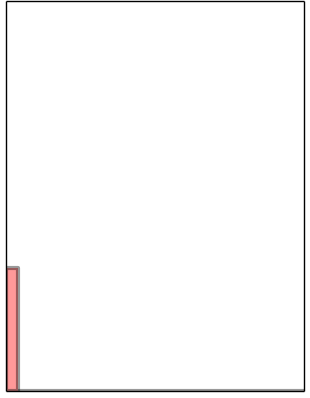
\includegraphics[scale=0.1]{images/module5/p1.png}};
		\node (plot) at (7.7,4.5) {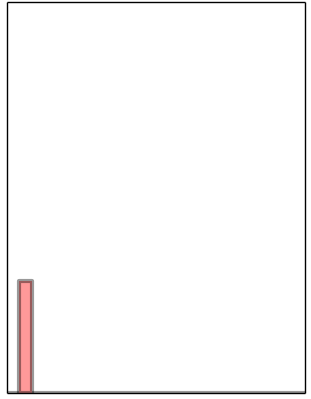
\includegraphics[scale=0.1]{images/module5/p2.png}};
		\node[text width=0.5cm] at (9.5,4) {\LARGE {.}};
		\node[text width=0.5cm] at (10.5,4) {\LARGE {.}};
		\node[text width=0.5cm] at (11.5,4) {\LARGE {.}};
		\node (plot) at (12.7,4.5) {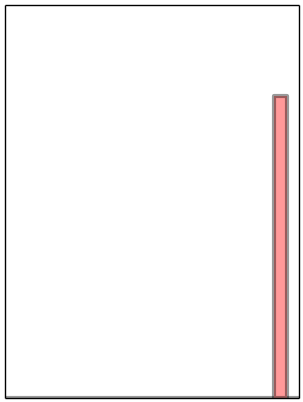
\includegraphics[scale=0.1]{images/module5/p3.png}};
		\node (plot) at (14.7,4.5) {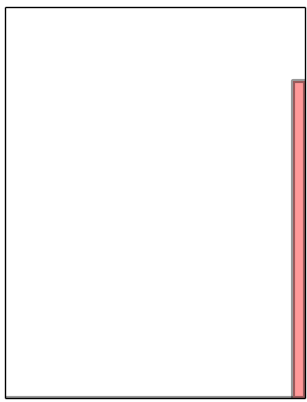
\includegraphics[scale=0.1]{images/module5/p4.png}};
	}

	\onslide<6-> {
		\node [neuron1] (neuron2) at (10,7) {$+$};
		\draw[->]  (5.7,5.4) -- (neuron2);
		\draw[->]  (7.7,5.4) -- (neuron2);

		\node[text width=0.5cm] at (9.5,5.5) {\LARGE {.}};
		\node[text width=0.5cm] at (10.5,5.5) {\LARGE {.}};
		\node[text width=0.5cm] at (11.5,5.5) {\LARGE {.}};

		\draw[->]  (12.7,5.4) -- (neuron2);
		\draw[->]  (14.7,5.4) -- (neuron2);
		\draw[->]  (neuron2) -- (10,8.8) ;
	}
	\node (plot) at (10,10.5) {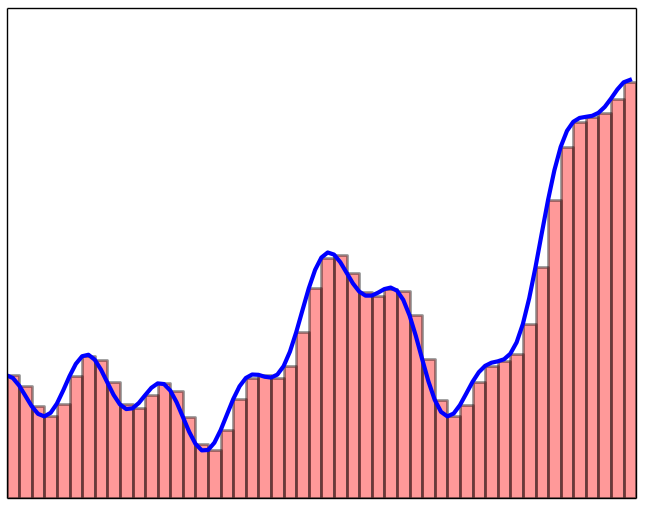
\includegraphics[width=7cm, height=2cm]{images/module5/plot.png}};
\end{tikzpicture}
		\end{overlayarea}
		\column{0.5\textwidth}
		\begin{overlayarea}{\textwidth}{\textheight}
			\begin{itemize}\justifying
				\item<1-> We make a few observations
				\item<2-> All these ``tower'' functions are similar and only differ in their heights and positions on the x-axis
				\item<3-> Suppose there is a black box which takes the original input ($x$) and constructs these tower functions
				\item<5-> We can then have a simple network which can just add them up to approximate the function
				\item<7-> Our job now is to figure out what is inside this blackbox
			\end{itemize}
		\end{overlayarea}
	\end{columns}
\end{frame}


\begin{frame}
	We will figure this out over the next few slides ...
\end{frame}

\begin{frame}
	\begin{columns}
		\column{0.5\textwidth}
		\begin{overlayarea}{\textwidth}{\textheight}
			\begin{onlyenv}
				\only<0-44>{
					\begin{figure}
						\includegraphics<1-2>[scale=0.25]{images/module5/Plots/sig_2d/a_6}
						\foreach \n in {0,...,44} {%
								\pgfmathsetmacro\result{int(\n + 6)}
								\pgfmathsetmacro\t{int(\n + 3)}
								\includegraphics<\t>[scale=0.25]{images/module5/Plots/sig_2d/a_\result}
							}
					\end{figure}
					\foreach \n in {0,...,44} {%
							\pgfmathsetmacro\result{int(\n + 6)}
							\pgfmathsetmacro\t{int(\n + 3)}
							\only<\t>{$\sigma(x) = \frac{1}{1- e^{-(wx + b)}}$ $w = \n, b = 0 $}
						}
				}
				\only<45->{
					\begin{figure}
						\foreach \n in {1,...,35} {%
								\pgfmathsetmacro\result{int(\n + 44)}
								\includegraphics<\result>[scale=0.25]{images/module5/Plots/sig_2d/b_\n}
							}
					\end{figure}
					\foreach \n in {1,...,35} {%
							\pgfmathsetmacro\result{int(\n + 44)}
							\only<\result>{$\sigma(x) = \frac{1}{1- e^{-(wx + b)}}$ $w = 50, b = \n $}
						}
				}
			\end{onlyenv}
		\end{overlayarea}
		\column{0.5\textwidth}
		\begin{overlayarea}{\textwidth}{\textheight}
			\begin{itemize}\justifying
				\item<1-> If we take the logistic function and set $w$ to a very high value we will recover the step function
				\item<2-> Let us see what happens as we change the value of $w$
				\item<45-> Further we can adjust the value of $b$ to control the position on the x-axis at which the function transitions from 0 to 1
			\end{itemize}
		\end{overlayarea}
	\end{columns}
\end{frame}

\begin{frame}
	\begin{columns}
		\column{0.5\textwidth}
		\begin{overlayarea}{\textwidth}{\textheight}
			\begin{tikzpicture}
	\node (plot) at (0,10) {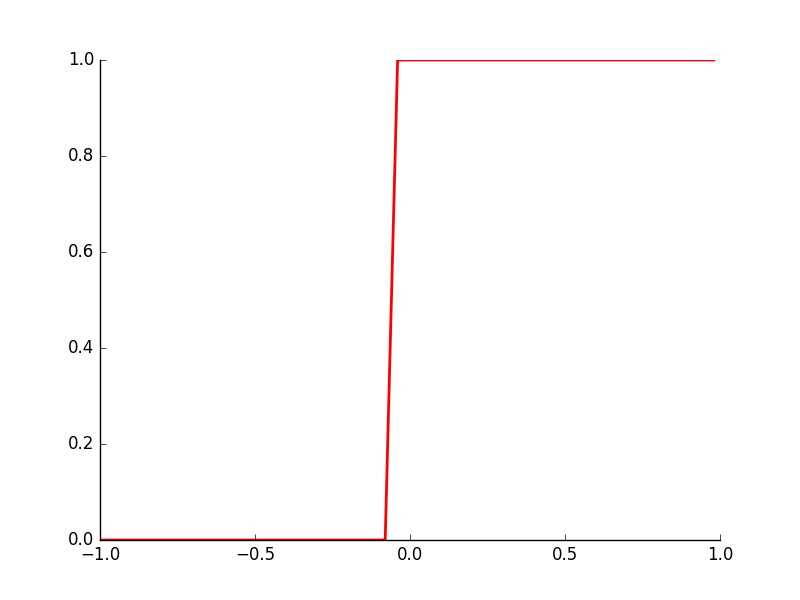
\includegraphics[width=4cm,height=4cm]{./images/module5/Plots/1}};

	\node (plot) at (4,10) {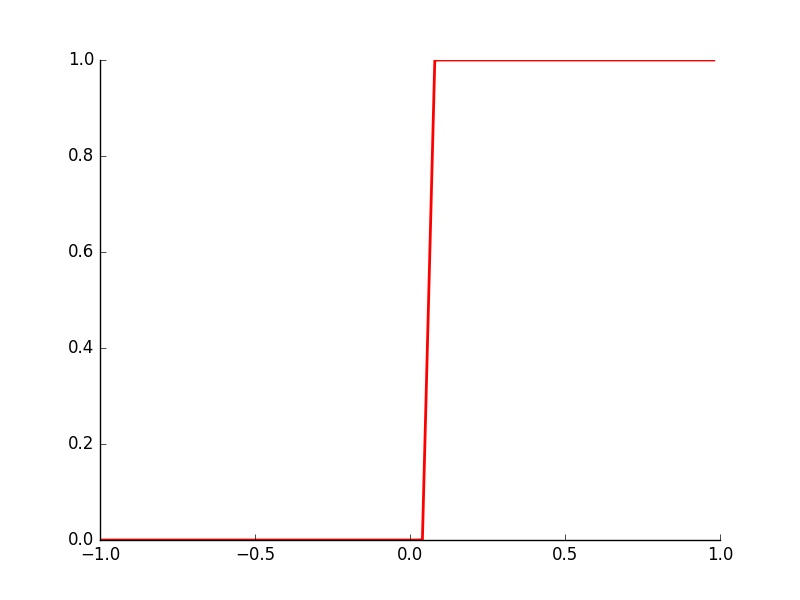
\includegraphics[width=4cm,height=4cm]{./images/module5/Plots/2}};

	\onslide<3->{\node (plot) at (2,6) {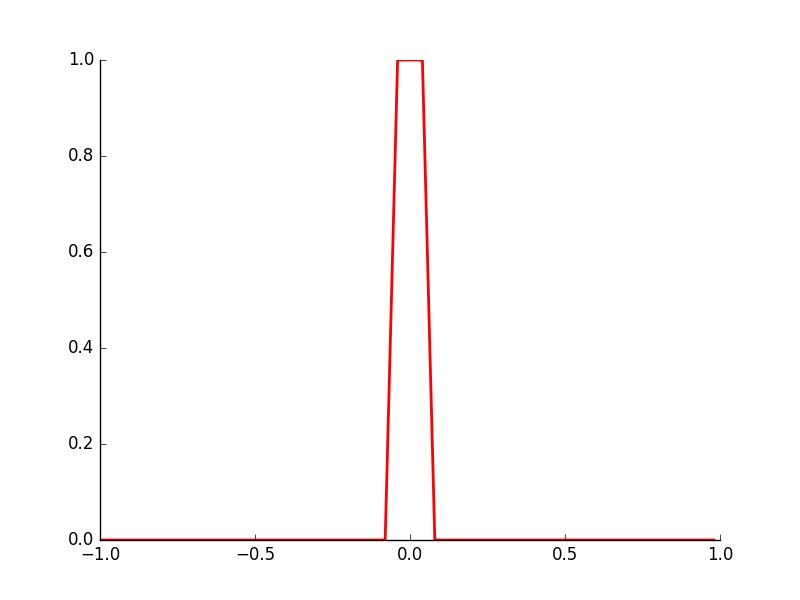
\includegraphics[width=4cm,height=4cm]{./images/module5/Plots/tower}};}
	\onslide<2->{\draw[line width=0.2mm](2, 10) -- (2.2,10);}
	%\draw[line width=0.2mm](2.1,10.1)--(2.1,9.9);
	\onslide<3->{\draw[line width=0.2mm](2,8) -- (2.2,8);}
	\onslide<3->{\draw[line width=0.2mm](2,8.1)--(2.2,8.1);}
\end{tikzpicture}
		\end{overlayarea}
		\column{0.5\textwidth}
		\begin{overlayarea}{\textwidth}{\textheight}
			\begin{itemize}\justifying
				\item Now let us see what we get by taking two such sigmoid functions (with different $b'$s) and subtracting one from the other
				\item<4-> Voila! We have our tower function !!
			\end{itemize}
		\end{overlayarea}
	\end{columns}
\end{frame}

\begin{frame}
	\begin{itemize}\justifying
		\item Can we come up with a neural network to represent this operation of subtracting one sigmoid function from another ?
	\end{itemize}
\end{frame}


\begin{frame}
	\begin{figure}
		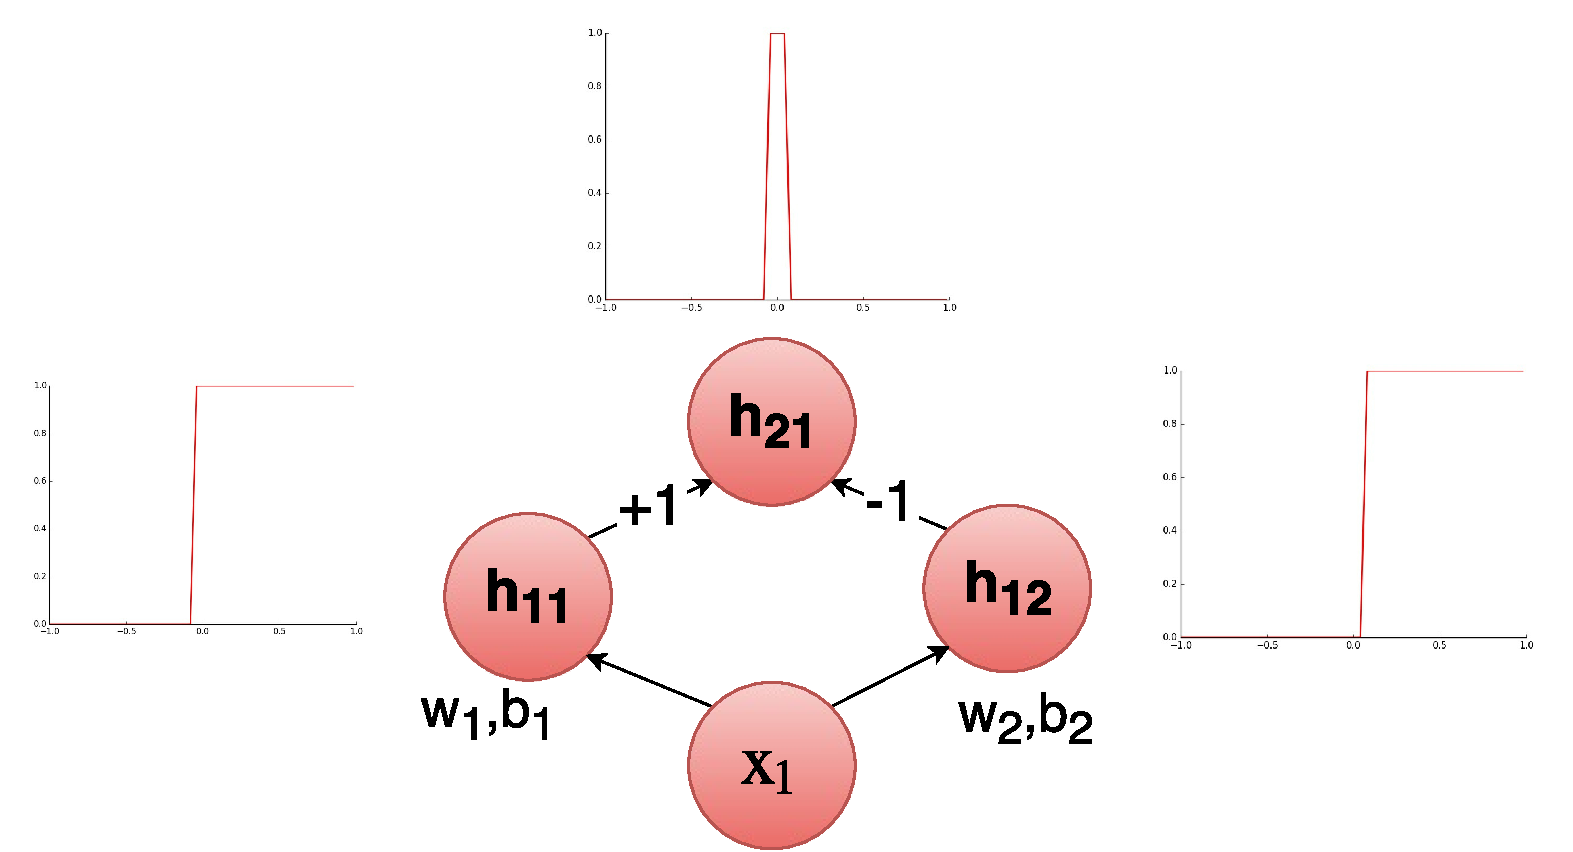
\includegraphics[scale=0.4]{images/module5/Plots/sig_add}
	\end{figure}
\end{frame}

\begin{frame}
	\begin{columns}
		\column{0.4\textwidth}
		\begin{overlayarea}{\textwidth}{\textheight}
			\begin{figure}
				\onslide<4->{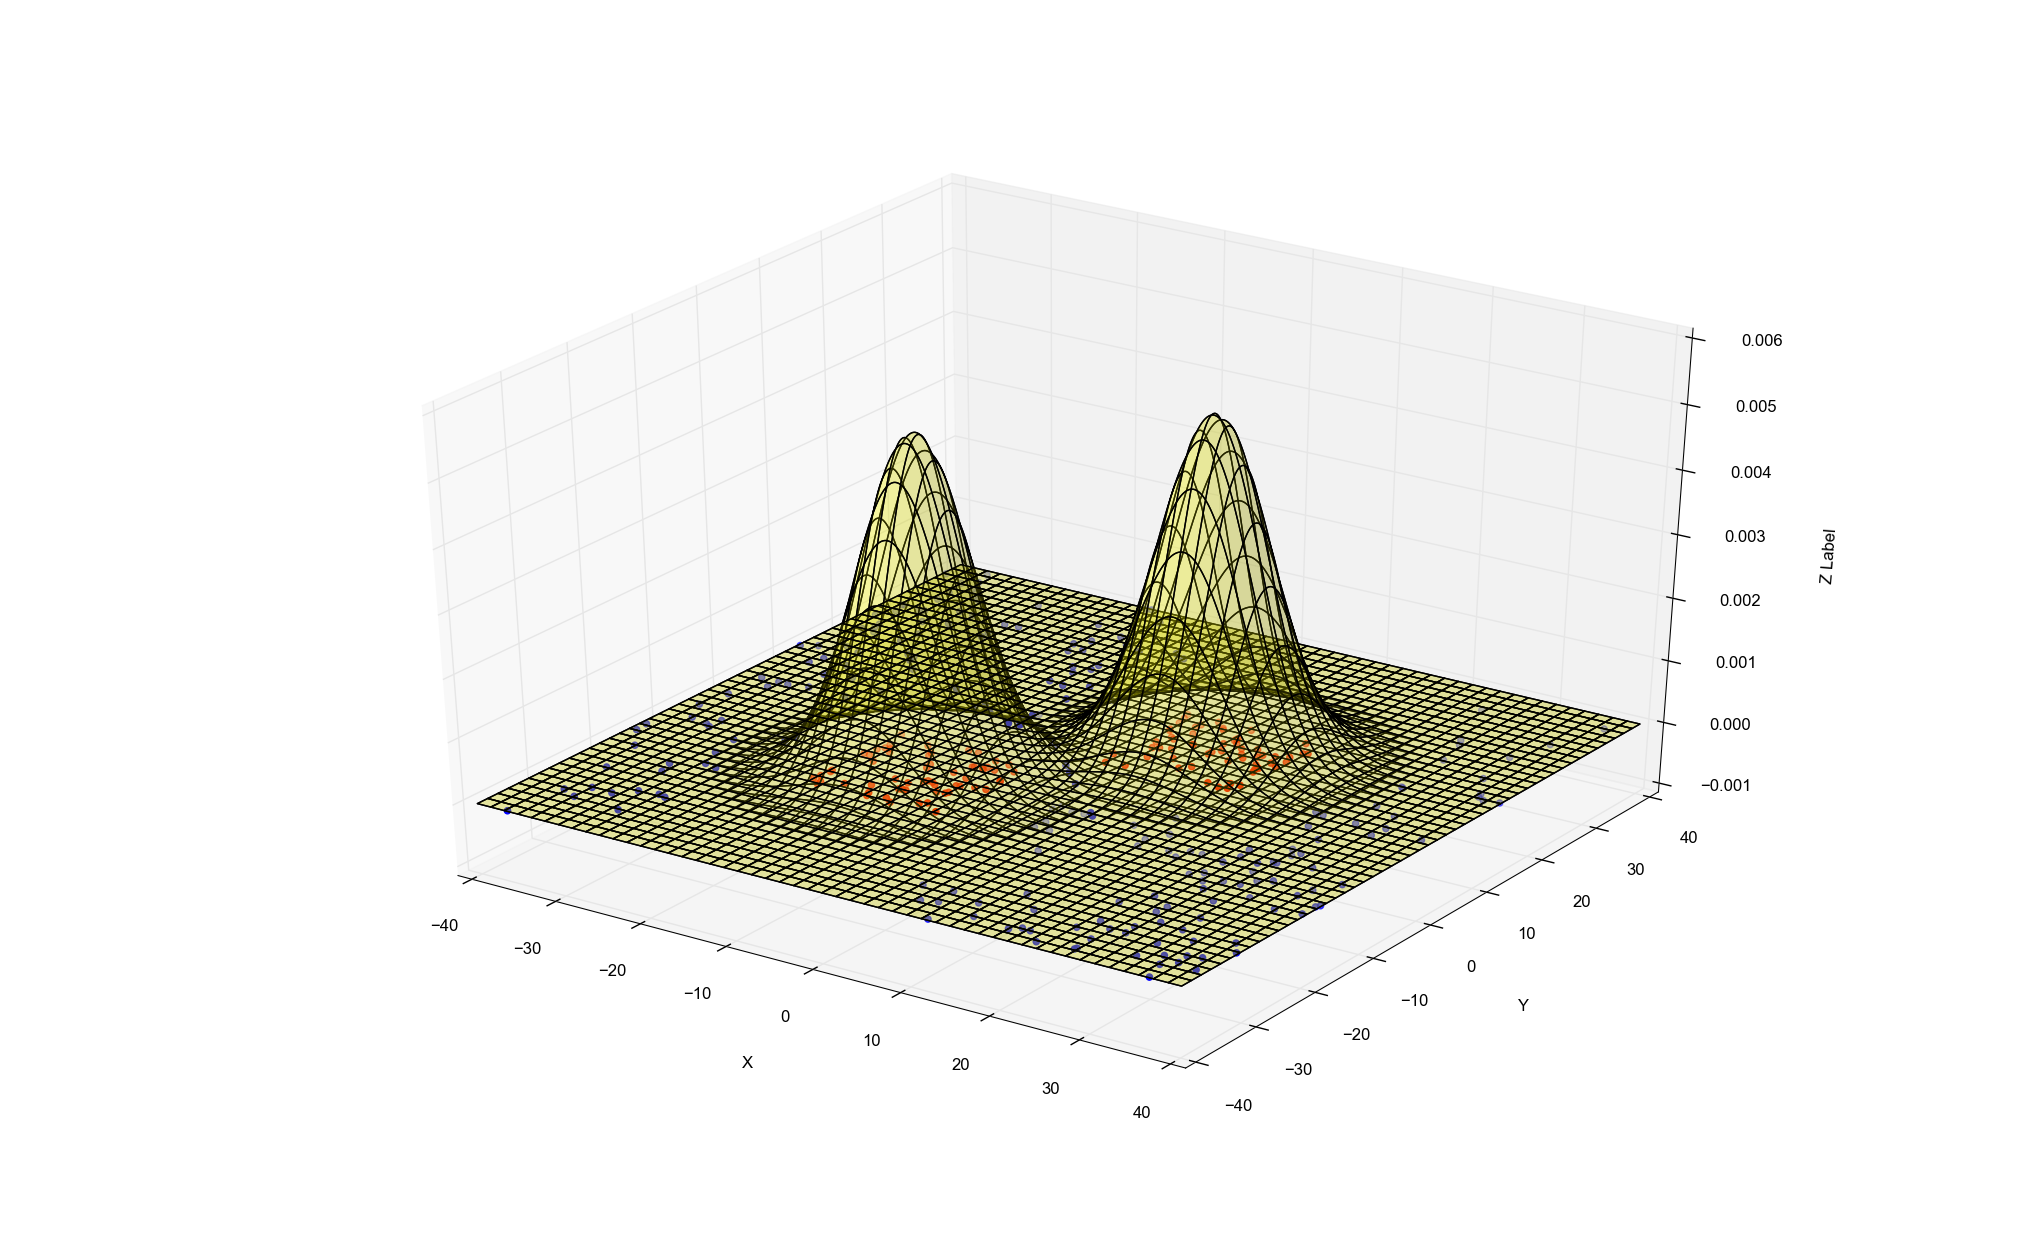
\includegraphics[scale=0.35]{images/module5/Plots/g2.png}}
			\end{figure}
		\end{overlayarea}
		\column{0.6\textwidth}
		\begin{overlayarea}{\textwidth}{\textheight}
			\begin{itemize}
			\item<1->{ What if we have more than one input?}
			\item<2-> {Suppose we are trying to take a decision about whether we will find oil at a particular location on the ocean bed(Yes/No)}
			\item<3-> {Further, suppose we base our decision on two factors: Salinity ($x_1$) and Pressure ($x_2$)}
			\item<4-> {We are given some data and it seems that $y(\text{oil}|\text{no-oil})$ is a complex function of $x_1$ and $x_2$}
			\item<5-> {We want a neural network to approximate this function}
			\end{itemize}
		\end{overlayarea}
	\end{columns}
\end{frame}

\begin{frame}
	\begin{columns}
		\column{0.5\textwidth}
		\begin{overlayarea}{\textwidth}{\textheight}
					\onslide<0->{
					\begin{align*}
						y &= \frac{1}{1 + e^{-(w_1x_1 + w_2x_2 + b)}}
					\end{align*}
			}
			\vspace{-0.3in}
			\begin{onlyenv}
				\only<0-26>{
					\begin{figure}
						\includegraphics<1-3>[scale=0.25]{images/module5/Plots/one/2}
						\foreach \n in {4,...,26} {%
								\pgfmathsetmacro\result{int(\n - 1)}
								\includegraphics<\n>[scale=0.25]{images/module5/Plots/one/\result}
							}

					\end{figure}
					\vspace{-0.3in}
						\foreach \n in {3,...,25} {%
							\pgfmathsetmacro\result{int(\n - 1)}
							\only<\n>{$w_1 = \result, w_2 = 0, b = 0 $}
						}
				}
			\end{onlyenv}
				%\vspace{-0.1in}


		\end{overlayarea}
		\column{0.5\textwidth}
		\begin{overlayarea}{\textwidth}{\textheight}
			\begin{itemize}\justifying
				\item<1-> This is what a 2-dimensional sigmoid looks like
				\item<2-> We need to figure out how to get a tower in this case
				\item<3-> First, let us set $w_2$ to 0 and see if we can get a two dimensional step function
				\item<26-> What would happen if we change $b$ ?
			\end{itemize}
		\end{overlayarea}
	\end{columns}
\end{frame}

\begin{frame}
	\begin{columns}
		\column{0.5\textwidth}
			\begin{overlayarea}{\textwidth}{\textheight}
					\begin{align*}
						y &= \frac{1}{1 + e^{-(w_1x_1 + w_2x_2 + b)}}
					\end{align*}
				\vspace{-0.3in}
				\begin{onlyenv}
				\only<0->{
					\begin{figure}
						\foreach \n in {0,...,9} {%
								\pgfmathsetmacro\result{int(\n + 0)}
								\includegraphics<\result>[scale=0.25]{images/module5/Plots/two/\n}
							}
					\end{figure}
					\vspace{-0.3in}
						\foreach \n in {0,...,9} {%
							\pgfmathsetmacro\result{int(\n + 0)}
							\pgfmathsetmacro\b{int(\n * 5)}
							\only<\result>{$w_1 = 25, w_2 = 0, b = \b $}
						}
				}
			\end{onlyenv}



		\end{overlayarea}
		\column{0.5\textwidth}
		\begin{overlayarea}{\textwidth}{\textheight}
			\begin{itemize}\justifying
				\item This is what a 2-dimensional sigmoid looks like
				\item We need to figure out how to get a tower in this case
				\item First, let us set $w_2$ to 0 and see if we can get a two dimensional step function
				\item What would happen if we change $b$ ?
			\end{itemize}
		\end{overlayarea}
	\end{columns}
\end{frame}

\begin{frame}
	\begin{columns}
		\column{0.5\textwidth}
		\begin{overlayarea}{\textwidth}{\textheight}
			\begin{tikzpicture}
	\node (plot) at (0,10) {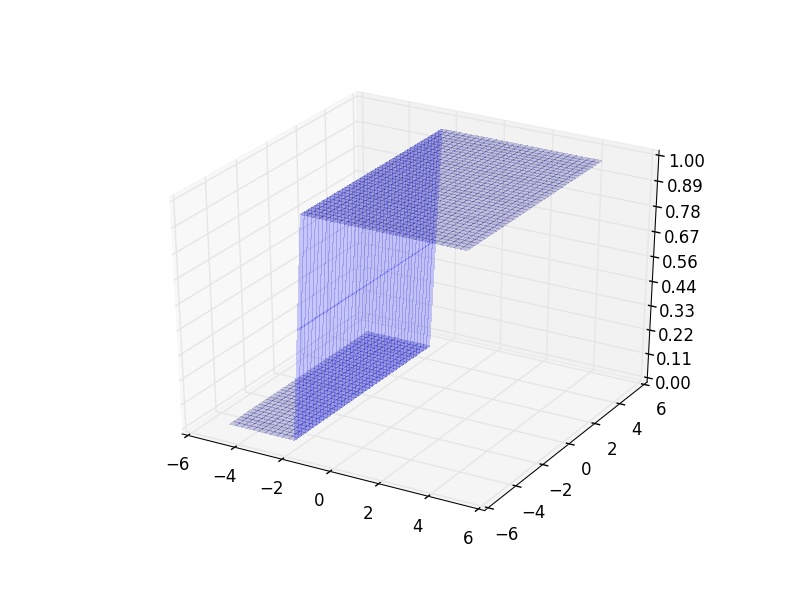
\includegraphics[width=4cm,height=4cm]{./images/module5/Plots/three/x1}};

	\node (plot) at (4,10) {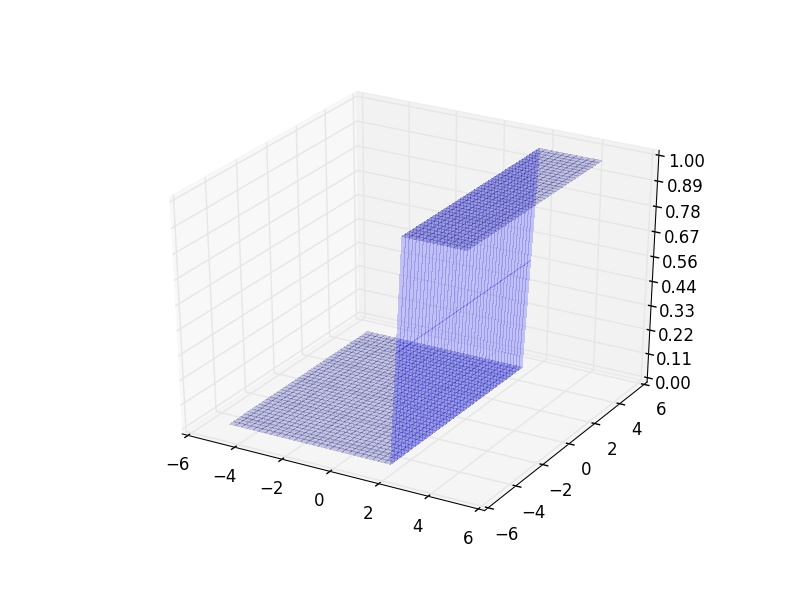
\includegraphics[width=4cm,height=4cm]{./images/module5/Plots/three/x2}};

	\onslide<3->{\node (plot) at (2,6) {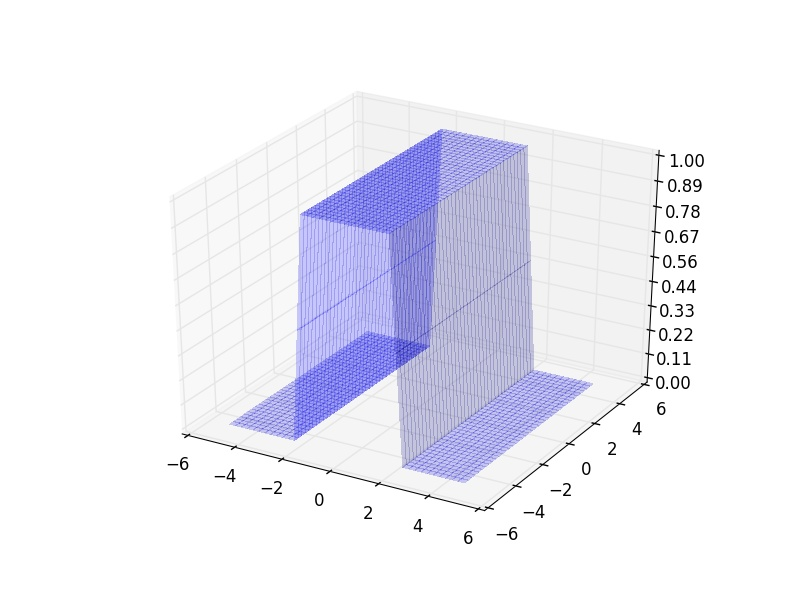
\includegraphics[width=4cm,height=4cm]{./images/module5/Plots/three/xjoin}};}
	\onslide<2->{\draw[line width=0.2mm](2, 10) -- (2.2,10);}
	%\draw[line width=0.2mm](2.1,10.1)--(2.1,9.9);
	\onslide<3->{\draw[line width=0.2mm](2,8) -- (2.2,8);}
	\onslide<3->{\draw[line width=0.2mm](2,8.1)--(2.2,8.1);}
\end{tikzpicture}
		\end{overlayarea}
		\column{0.5\textwidth}
		\begin{overlayarea}{\textwidth}{\textheight}
			\begin{itemize}\justifying
				\item<1-> What if we take two such step functions (with different $b$ values) and subtract one from the other
				\item<4-> We still don't get a tower (or we get a tower which is open from two sides)
			\end{itemize}
		\end{overlayarea}
	\end{columns}
\end{frame}

\begin{frame}
	\begin{columns}
		\column{0.5\textwidth}
		\begin{overlayarea}{\textwidth}{\textheight}
			\only<0->{
				\begin{align*}
					y &= \frac{1}{1 + e^{-(w_1x_1 + w_2x_2 + b)}}
				\end{align*}
			}
			\vspace{-0.3in}
			\begin{onlyenv}
				\only<0-26>{
					\begin{figure}
						\includegraphics<1-3>[scale=0.25]{images/module5/Plots/five/2}
						\foreach \n in {4,...,26} {%
								\pgfmathsetmacro\result{int(\n - 1)}
								\includegraphics<\n>[scale=0.25]{images/module5/Plots/five/\result}
							}
					\end{figure}
					\vspace{-0.3in}
					\foreach \n in {3,...,25} {%
							\pgfmathsetmacro\result{int(\n - 1)}
							\only<\n>{$w_1 = 0, w_2 = \result, b = 0 $}
						}
				}
			\end{onlyenv}
		\end{overlayarea}
		\column{0.5\textwidth}
		\begin{overlayarea}{\textwidth}{\textheight}
			\begin{itemize}\justifying
				\item<1-> Now let us set $w_1$ to 0 and adjust $w_2$ to get a 2-dimensional step function with a different orientation
				\item<26-> And now we change $b$
			\end{itemize}
		\end{overlayarea}
	\end{columns}
\end{frame}

\begin{frame}
	\begin{columns}
		\column{0.5\textwidth}
		\begin{overlayarea}{\textwidth}{\textheight}
			\only<0->{
				\begin{align*}
					y &= \frac{1}{1 + e^{-(w_1x_1 + w_2x_2 + b)}}
				\end{align*}
			}
			\vspace{-0.3in}
			\begin{onlyenv}
				\only<0->{
					\begin{figure}
						\foreach \n in {0,...,9} {%
								\pgfmathsetmacro\result{int(\n + 0)}
								\includegraphics<\result>[scale=0.25]{images/module5/Plots/six/\n}
							}
					\end{figure}
					\vspace{-0.3in}
					\foreach \n in {0,...,9} {%
							\pgfmathsetmacro\result{int(\n + 0)}
							\pgfmathsetmacro\b{int(\n * 5)}
							\only<\result>{$w_1 = 0, w_2 = 25, b = \b $}
						}
				}
			\end{onlyenv}
		\end{overlayarea}
		\column{0.5\textwidth}
		\begin{overlayarea}{\textwidth}{\textheight}
			\begin{itemize}\justifying
				\item<1-> Now let us set $w_1$ to 0 and adjust $w_2$ to get a 2-dimensional step function with a different orientation
				\item<1-> And now we change $b$
			\end{itemize}
		\end{overlayarea}
	\end{columns}
\end{frame}

\begin{frame}
	\begin{columns}
		\column{0.5\textwidth}
		\begin{overlayarea}{\textwidth}{\textheight}
			\begin{tikzpicture}

	\node (plot) at (0,10) {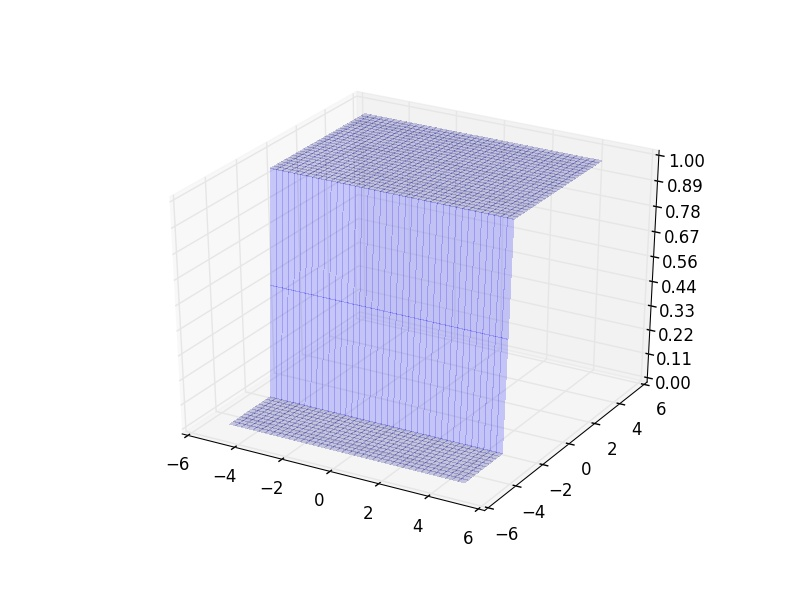
\includegraphics[width=4cm,height=4cm]{./images/module5/Plots/three/y1}};

	\node (plot) at (4,10) {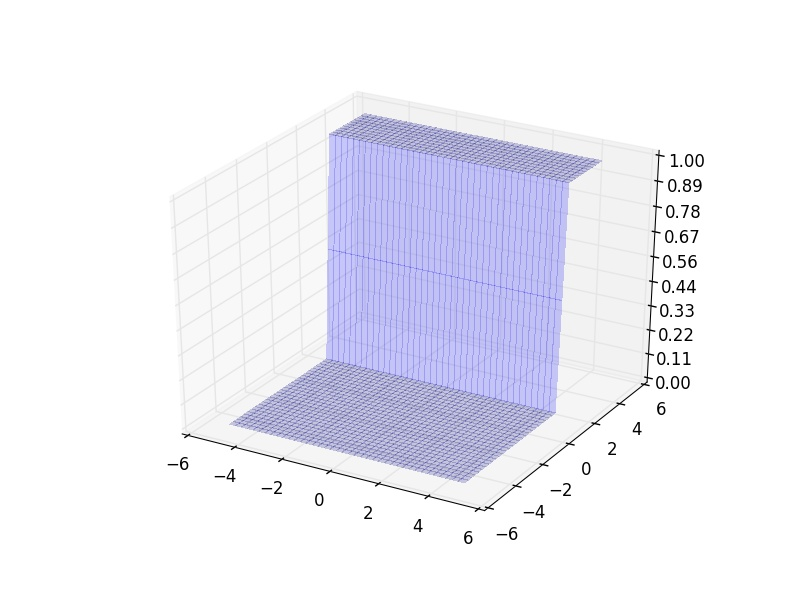
\includegraphics[width=4cm,height=4cm]{./images/module5/Plots/three/y2}};

	\onslide<3->{\node (plot) at (2,6) {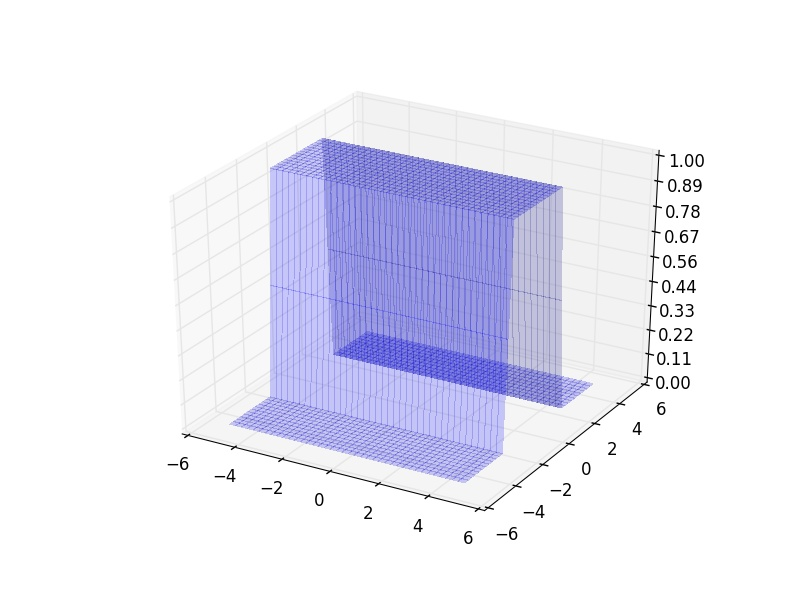
\includegraphics[width=4cm,height=4cm]{./images/module5/Plots/three/yjoin}};}
	\onslide<2->{\draw[line width=0.2mm](2, 10) -- (2.2,10);}
	%\draw[line width=0.2mm](2.1,10.1)--(2.1,9.9);
	\onslide<3->{\draw[line width=0.2mm](2,8) -- (2.2,8);}
	\onslide<3->{\draw[line width=0.2mm](2,8.1)--(2.2,8.1);}
\end{tikzpicture}
		\end{overlayarea}
		\column{0.5\textwidth}
		\begin{overlayarea}{\textwidth}{\textheight}
			\begin{itemize}\justifying
				\item<1-> Again, what if we take two such step functions (with different $b$ values) and subtract one from the other
				\item<4-> We still don't get a tower (or we get a tower which is open from two sides)
				\item<5-> Notice that this open tower has a different orientation from the previous one
			\end{itemize}
		\end{overlayarea}
	\end{columns}
\end{frame}

\begin{frame}
	\begin{columns}
		\column{0.5\textwidth}
		\begin{overlayarea}{\textwidth}{\textheight}
			\only<1-5>{
				\begin{tikzpicture}
	\node (plot) at (0,10) {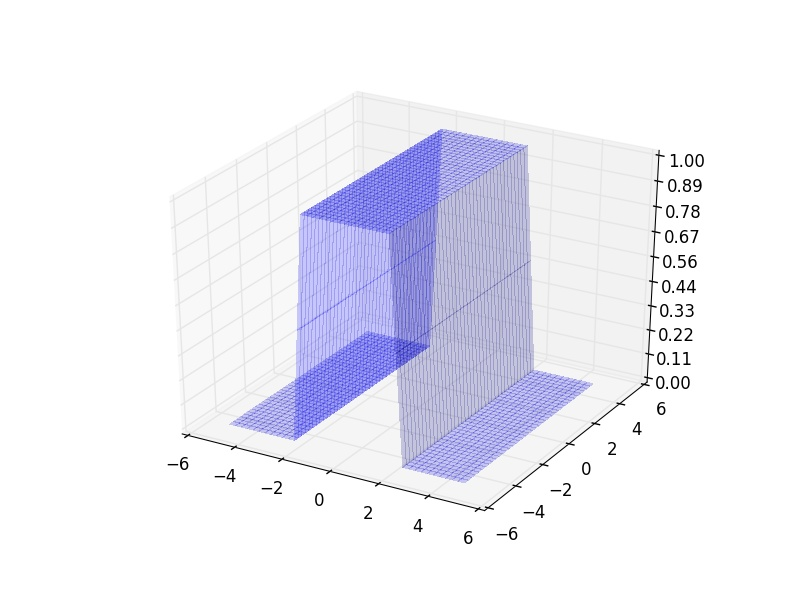
\includegraphics[width=4cm,height=4cm]{./images/module5/Plots/three/xjoin}};

	\node (plot) at (4,10) {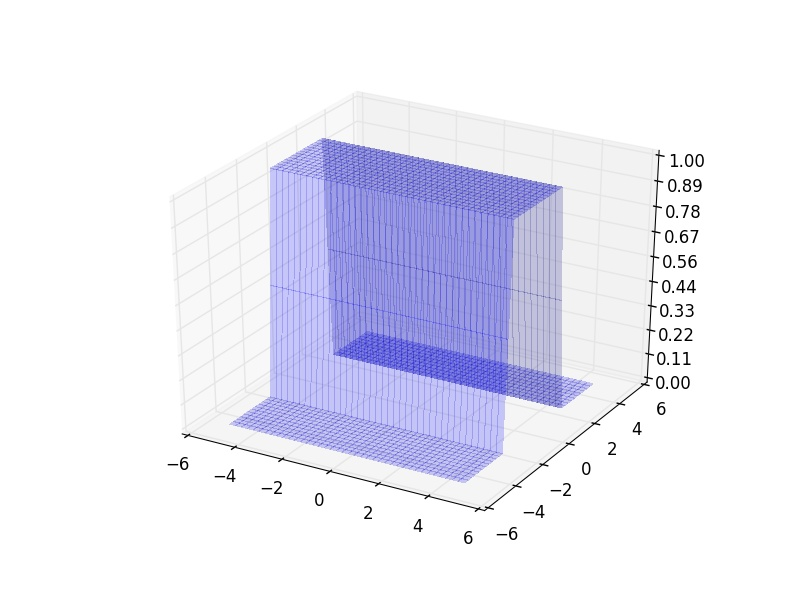
\includegraphics[width=4cm,height=4cm]{./images/module5/Plots/three/yjoin}};

	\onslide<3->{\node (plot) at (2,6) {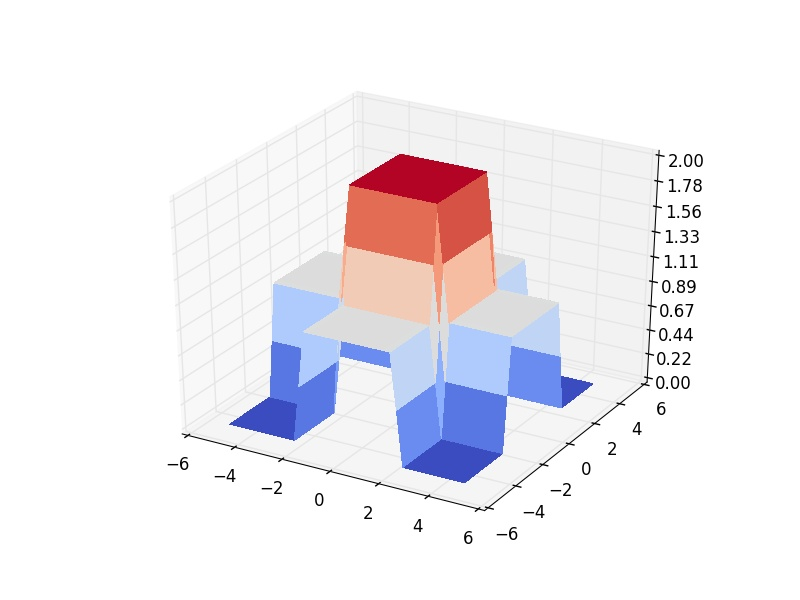
\includegraphics[width=4cm,height=4cm]{./images/module5/Plots/three/xpyjoin}};}
	\onslide<2->{\draw[line width=0.2mm](2, 10) -- (2.2,10);}
	%\draw[line width=0.2mm](2.1,10.1)--(2.1,9.9);
	\onslide<3->{\draw[line width=0.2mm](2,8) -- (2.2,8);}
	\onslide<3->{\draw[line width=0.2mm](2,8.1)--(2.2,8.1);}
\end{tikzpicture}
			}
			\only<6->{
				\begin{figure}
					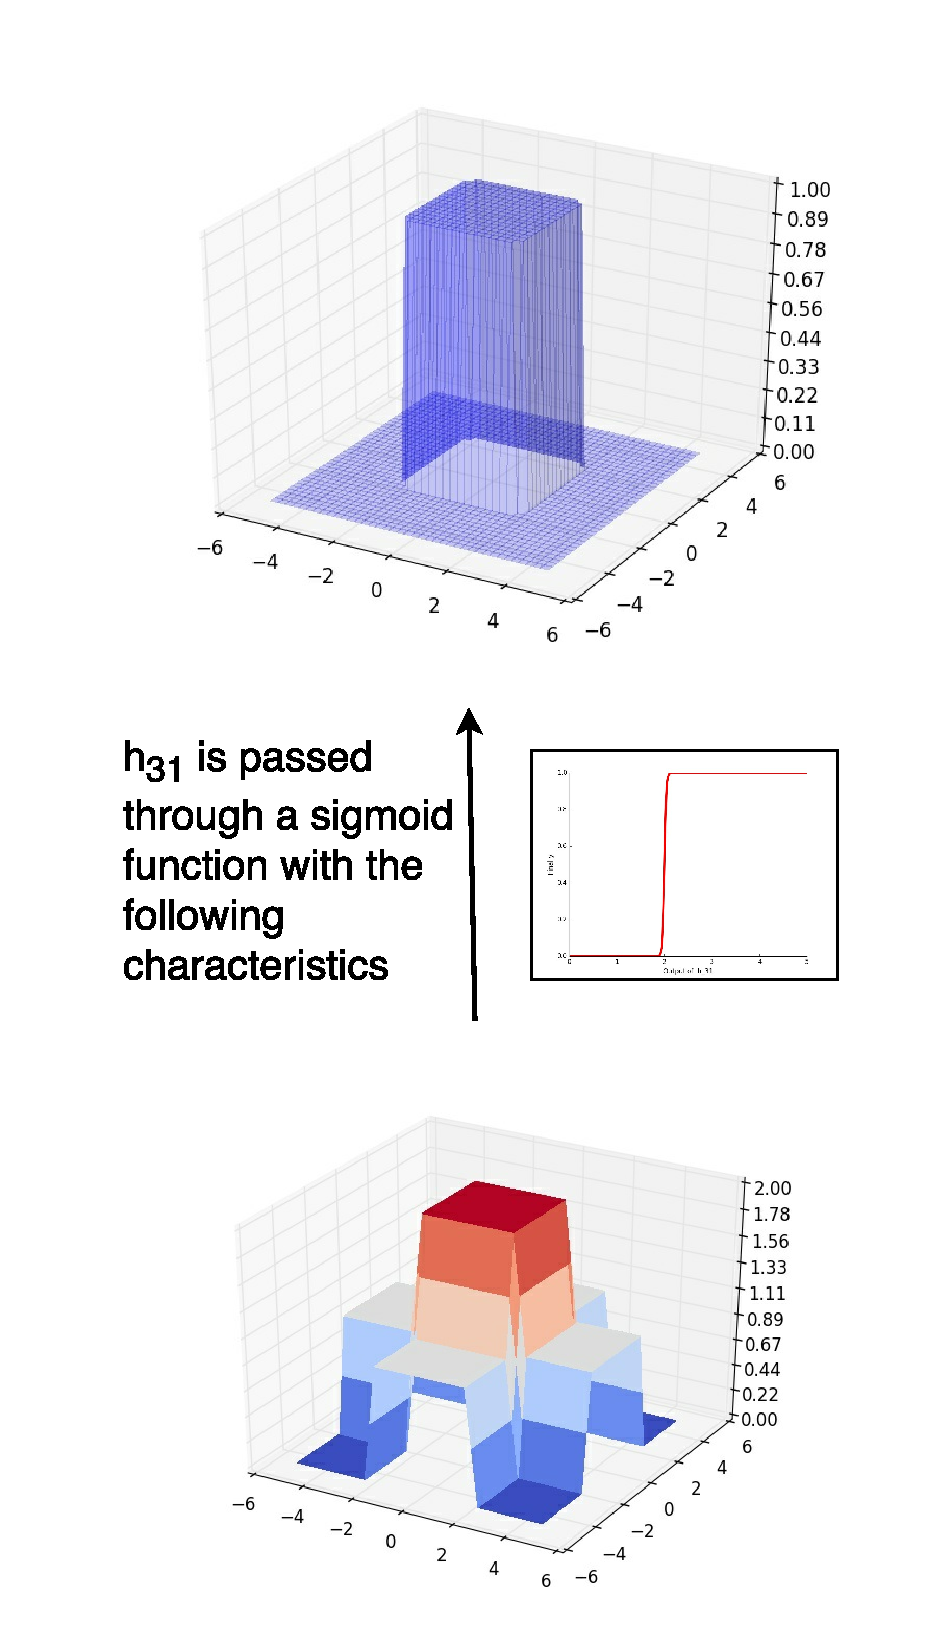
\includegraphics[scale=0.2]{./images/module5/Plots/tower_sigmoid}
				\end{figure}
			}
		\end{overlayarea}
		\column{0.5\textwidth}
		\begin{overlayarea}{\textwidth}{\textheight}
			\begin{itemize}\justifying
				\item<1-> Now what will we get by adding two such open towers ?
				\item<4-> We get a tower standing on an elevated base
				\item<5-> We can now pass this output through another sigmoid neuron to get the desired tower !
				\item<7-> We can now approximate any function by summing up many such towers
			\end{itemize}
		\end{overlayarea}
	\end{columns}
\end{frame}

\begin{frame}
	\begin{columns}
		\column{0.5\textwidth}
		\begin{overlayarea}{\textwidth}{\textheight}
			\begin{figure}
				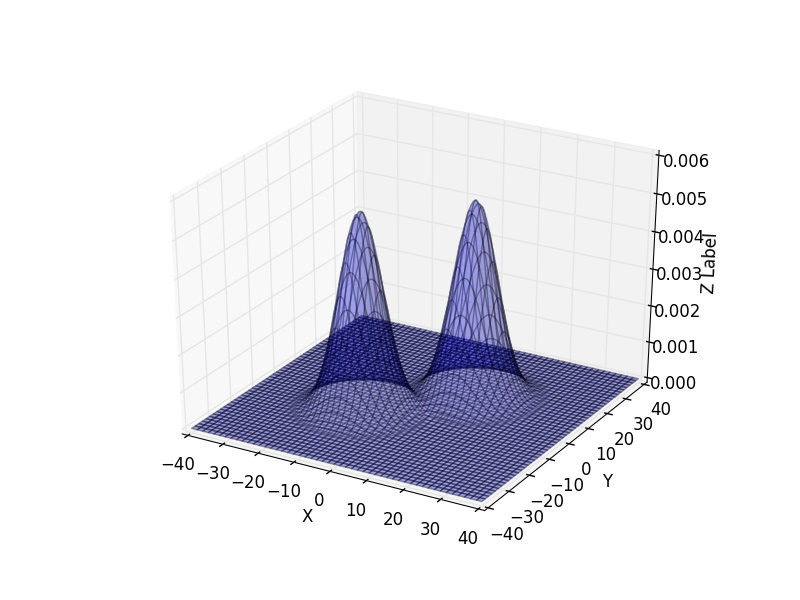
\includegraphics[scale=0.25]{images/module5/Plots/2bells}
			\end{figure}
		\end{overlayarea}
		\column{0.5\textwidth}
		\begin{overlayarea}{\textwidth}{\textheight}
			\begin{itemize}\justifying
				\item For example, we could approximate the following function using a sum of several towers
			\end{itemize}
		\end{overlayarea}
	\end{columns}
\end{frame}

\begin{frame}
	\begin{itemize}\justifying
		\item Can we come up with a neural network to represent this entire procedure of constructing a 3 dimensional tower ?
	\end{itemize}
\end{frame}

\begin{frame}
	\begin{figure}
		\vspace{-0.2in}
		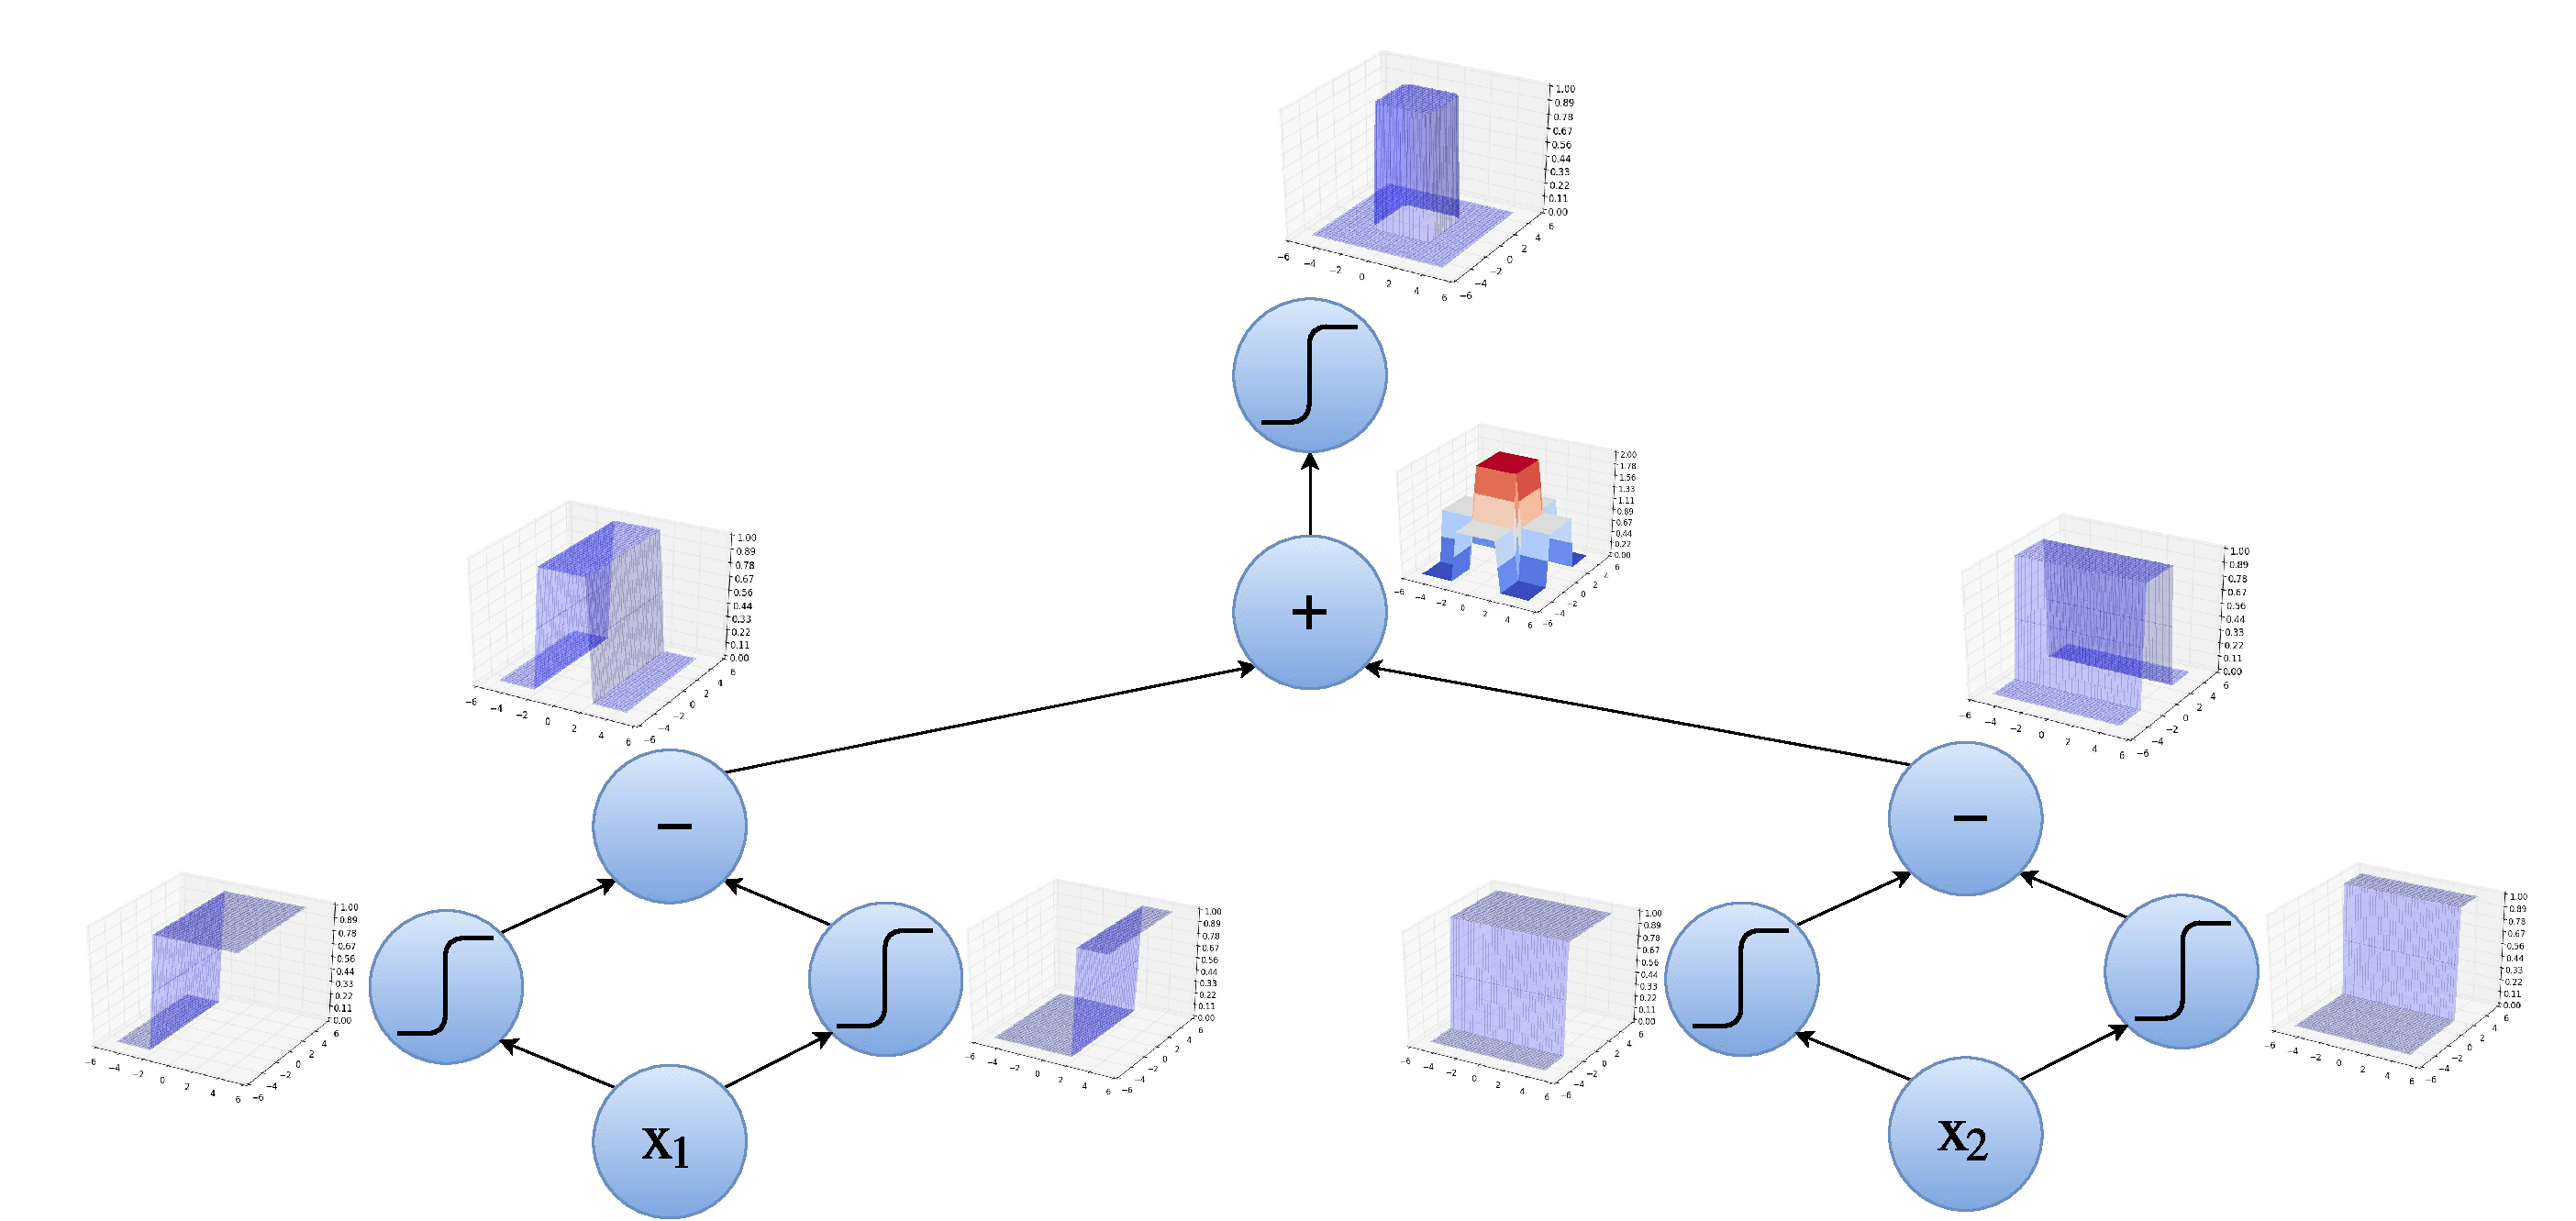
\includegraphics[scale=0.28]{images/module5/Plots/nn_step}
	\end{figure}
\end{frame}

\begin{frame}
	\begin{figure}
		\vspace{-0.2in}
		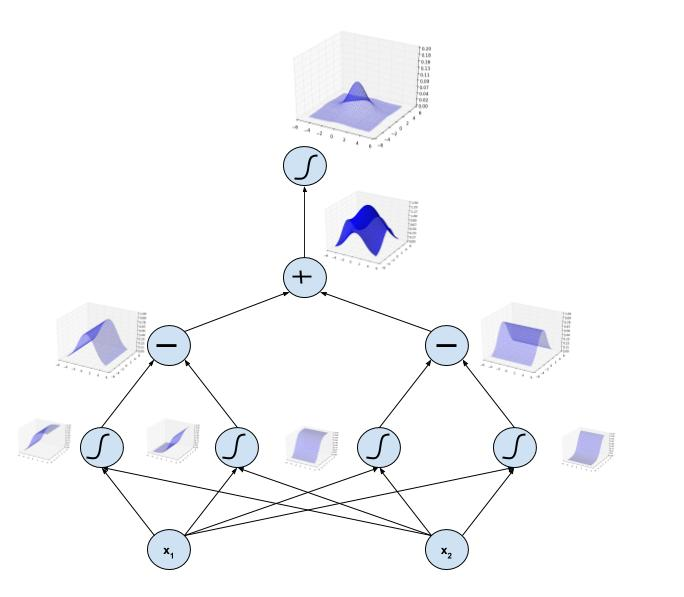
\includegraphics[scale=0.28]{images/module5/Plots/nn_g}
	\end{figure}
\end{frame}


\begin{frame}
	\begin{block}{Think}
		\begin{itemize}\justifying
			\item For 1 dimensional input we needed 2 neurons to construct a tower
			\item For 2 dimensional input we needed 4 neurons to construct a tower
			\item How many neurons will you need to construct a tower in $n$ dimensions ?
		\end{itemize}
	\end{block}
\end{frame}

\begin{frame}
	\begin{block}{Time to retrospect}
		\begin{itemize}\justifying
			\item Why do we care about approximating any arbitrary function ?
			\item Can we tie all this back to the classification problem that we have been dealing with ?
		\end{itemize}
	\end{block}
\end{frame}


\begin{frame}
	\begin{columns}
		\column{0.5\textwidth}
		\begin{overlayarea}{\textwidth}{\textheight}
			\begin{figure}
				\includegraphics<1-2>[scale=0.35]{images/module5/Plots/scatter.png}
				\includegraphics<3->[scale=0.35]{images/module5/Plots/sigmoid_plot.png}
			\end{figure}
			\vspace{-0.2in}
			\footnotesize{
			\begin{itemize}\justifying
				\item We are interested in separating the blue points from the red points
				\item<2-> Suppose we use a single sigmoidal neuron to approximate the relation between $x = [x_1, x_2]$ and $y$
				\item<4-> Obviously, there will be errors (some blue points get classified as 1 and some red points get classified as 0)
			\end{itemize}}
		\end{overlayarea}
		\column{0.5\textwidth}
		\begin{overlayarea}{\textwidth}{\textheight}
			\begin{figure}
				\includegraphics<5->[scale=0.35]{images/module5/Plots/g2.png}
			\end{figure}
			\vspace{-0.2in}
			\footnotesize{
			\begin{itemize}\justifying
				\item<5-> This is what we actually want
				\item<6-> The illustrative proof that we just saw tells us that we can have a neural network with two hidden layers which can approximate the above function by a sum of towers
				\item<7-> Which means we can have a neural network which can exactly separate the blue points from the red points !!
			\end{itemize}}
		\end{overlayarea}
	\end{columns}
\end{frame}
